\documentclass[tikz,border=5pt]{standalone}
\usepackage{tikz}

\begin{document}
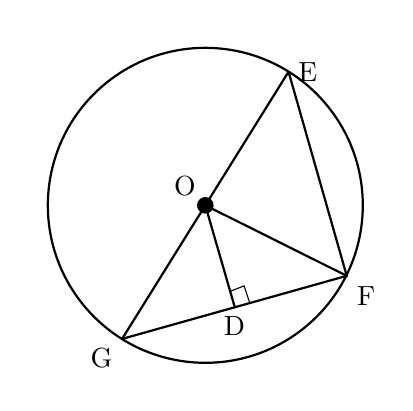
\begin{tikzpicture}[rotate=40, scale=2]

    \draw[thick] (0,0) circle (1);
    \node at (0,0) (O) {};
    \fill (0,0) circle (1.5pt) node[above left] {O};
    

    \draw[thick] (-0.95, -0.31) coordinate (G) -- (0.95, 0.31) coordinate (E);
    \node[below left] at (G) {G};
    \node[right] at (E) {E};

    \coordinate (F) at (0.4, -0.92);
    \draw[thick] (G) -- (F) -- (E);

    \coordinate (D) at (-0.27, -0.61);
    \draw[thick] (0,0) -- (D) node[below] {D};
    \draw[thick] (0,0) -- (F) node[below right] {F};

    \draw (-0.23, -0.52) -- (-0.14, -0.55) -- (-0.18, -0.65);

    % \node[scale=0.8] at (-0.7, -0.5) {4 cm};
    % \node[scale=0.8] at (0.3, 0.4) {10 cm};
\end{tikzpicture}

\end{document}
